\chapter{パーミッション}

\section*{セキュリティとファイルの共有}

「パーミッション -- permission」とは、「許可」という意味だ。

 UNIX システムでは、ファイルに 3 種類のパーミッションがある。
「ファイルを読む許可」「ファイルを書いたり消したりする許可」
「ファイルを実行する許可」の 3 つだ。

ユーザは自分のファイルに、この 3 種類のパーミッションを自由に設定できる。
この機能を使うと、自分で間違って大事なファイルを消さないように設定したり、
他人とファイルを共有したり、秘密のファイルを作ったりすることができる。

 UNIX システムでは、このパーミッションというしくみによって、
セキュリティを確保しつつ、他の人と一緒にプログラムを作ったりすることが
できるようになっている。

今回は、簡単なプログラムの作り方を説明しながら、
パーミッションの設定の仕方を紹介しよう。

\section{C プログラミング}

UNIX システムでプログラムを書くときには、
まず Mule をバックグラウンドなどにして他のウィンドウで起動する。
そして Mule を使って C などでソース・コード
\footnote{source code: 「(プログラムの)元になるコード」という意味。}
を書いてセーブする。
このとき、 Mule は終了しないで、ウィンドウを開きっぱなしにしておくとよい。

\begin{figure}[H]
\centering{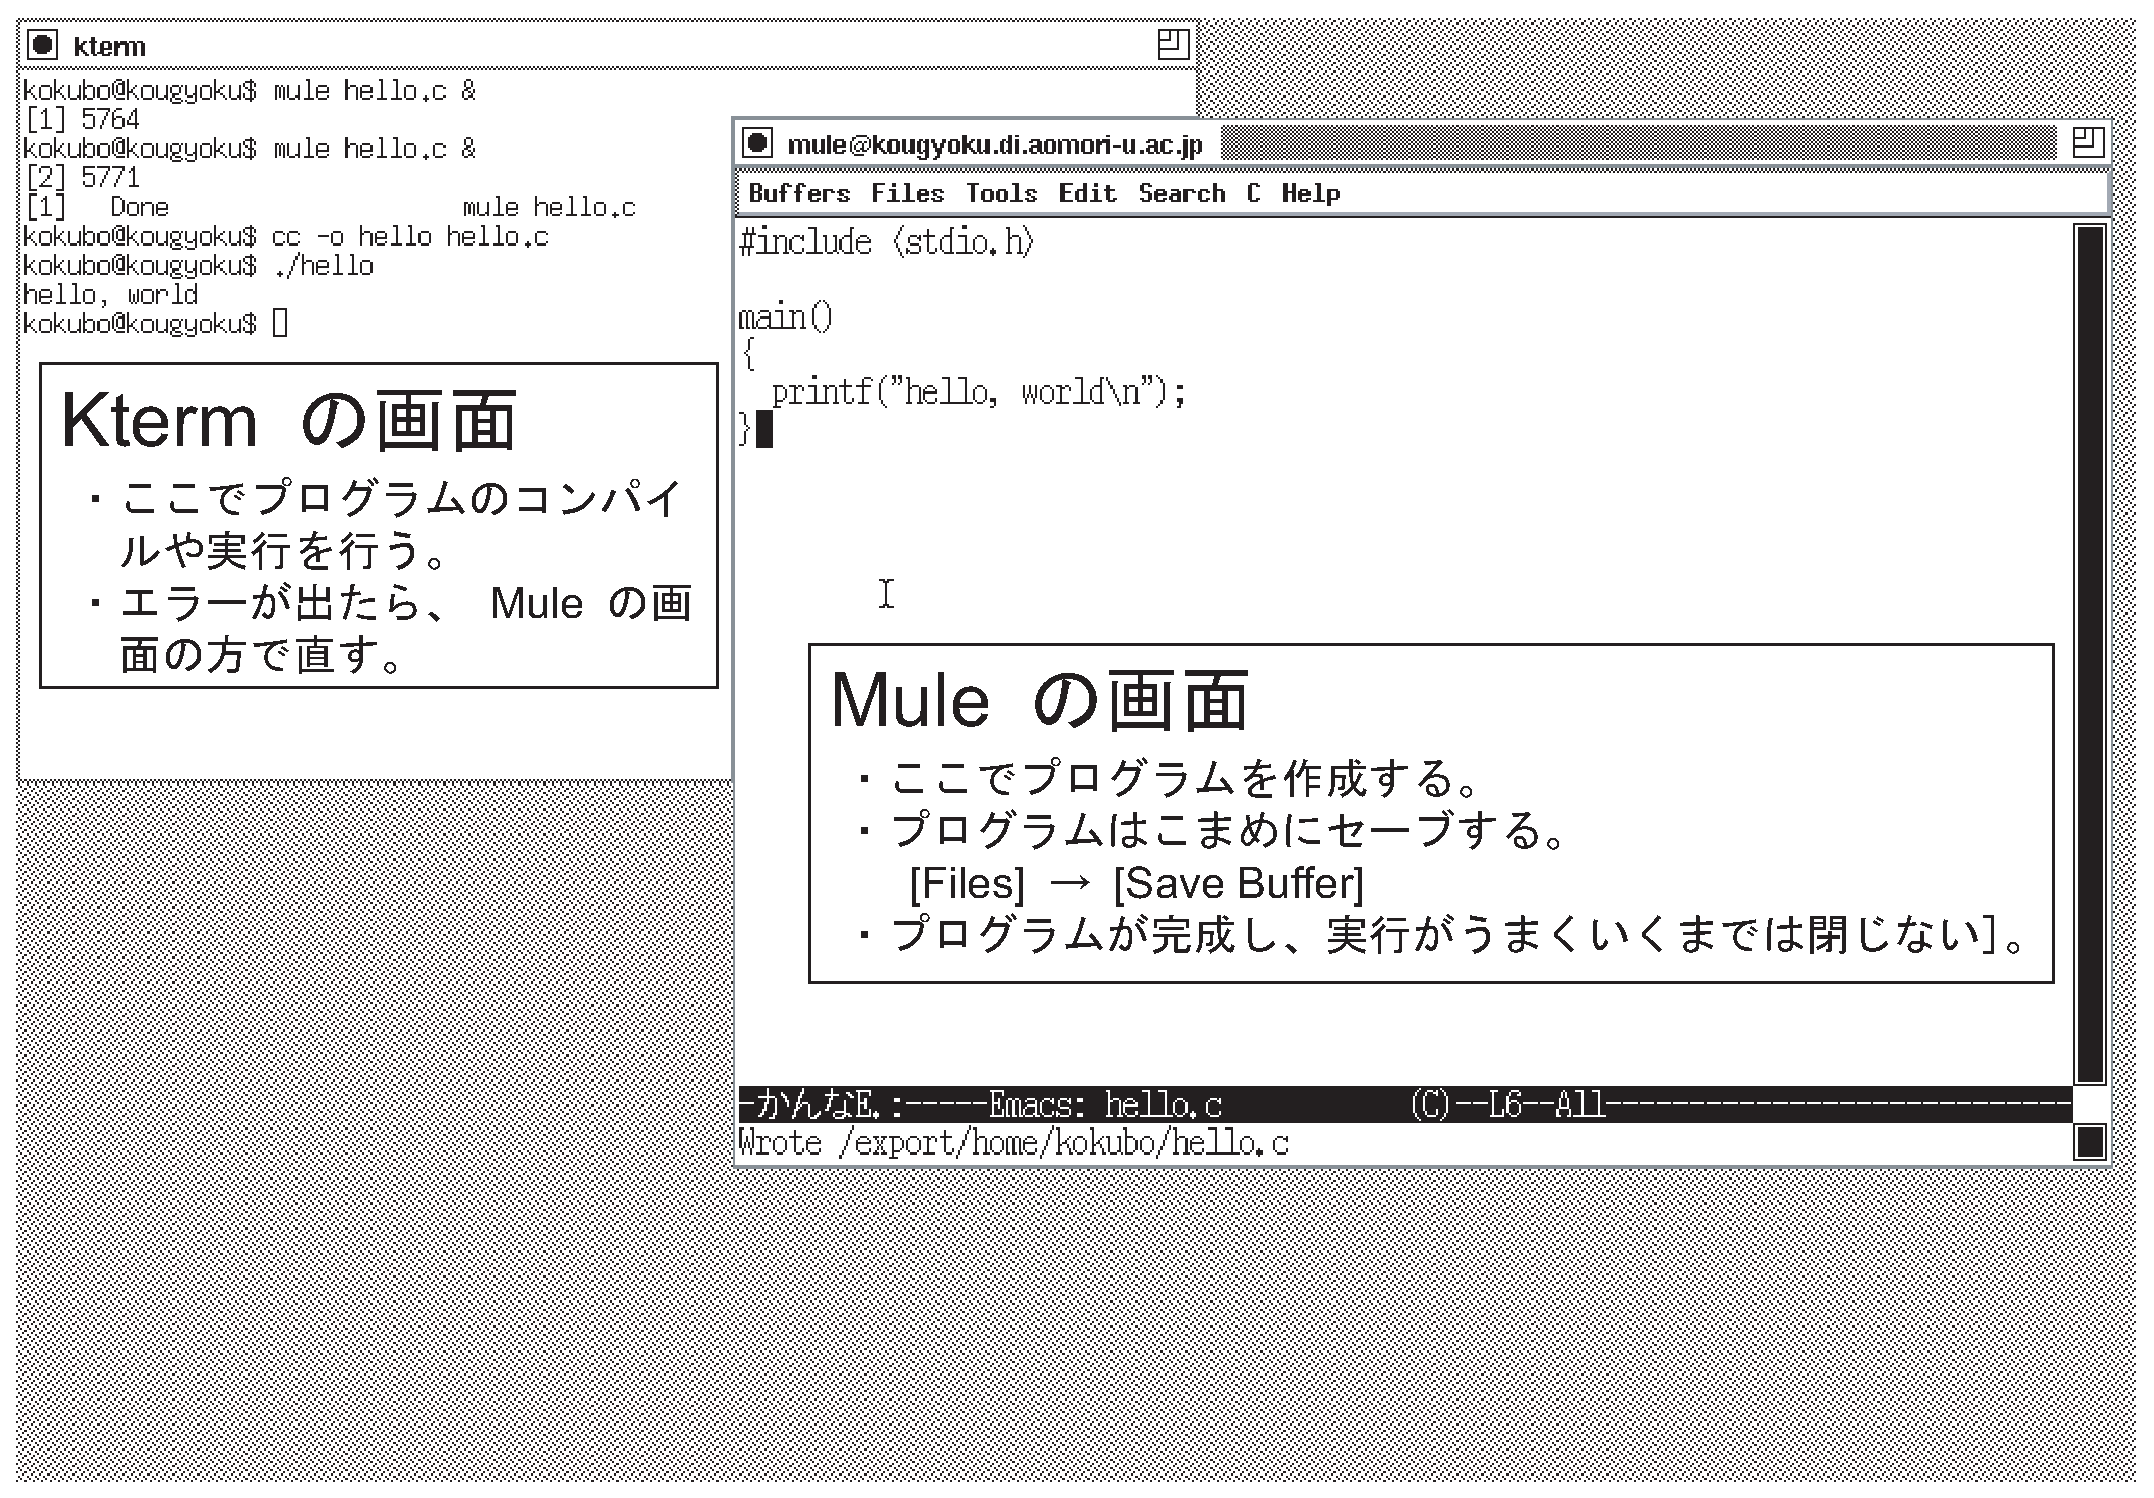
\includegraphics[scale=0.33]{progdevwin.eps}}
\end{figure}

それから、別のウィンドウでコンパイルするためのコマンドを打つ。
もしもエラーが出たら、 Mule のウィンドウに戻って修正し、
またセーブする。

そしてうまくコンパイルできたら、実行する。
すべてがうまくいくようになったら、 Mule のウィンドウを閉じて終わりにする。

\subsection{ソース・コードの作成}

では、実際に Mule でソース・コードを作成してみよう。

 C 言語のテキストの古典中の古典\footnote{個人的には、初心者にはあまりすすめない。}
と言えば、ブライアン・カーニハンと、 UNIX を開発したデニス・リッチーが
共同で書いた『プログラミング言語 C』(石田 晴久訳 共立出版)だろう。
この本の一番最初に載っている、「\texttt{hello, world}」と表示する
プログラムを作ってみよう。

まず、 Mule で「\texttt{hello.c}」いうファイルを作る。
 UNIX システムでは、 C のプログラムには、ファイル名の最後に
「\texttt{.c}」を付けるという約束があるので、このような名前を付ける。
自分でプログラムを書くときは、「なんとか\texttt{.c}」のような
感じの名前を付けるといい。

具体的には、次のように Mule を起動する。

\begin{progls}
% \slbfl{mule hello.c &}
\end{progls}

すると、 Mule が自動的に C モードで起動する
\footnote{ファイル名に「\texttt{.c}」が付いていると、
自動的に C モードになる。}。
なお、 C モードでは、プログラムの入力を助けてくれる機能が使えるが、
今回は紹介しない\footnote{実際には、ウィンドウを複数開かなくてもプログラムの作成、コンパイル、実行まで行なえる。}。

\bigskip

「\texttt{hello.c}」の中には、次のようなプログラムを書き、
 [Files] メニューから [Save Buffer] でセーブしよう。
このとき、 Mule はセーブするだけで終了はしない。

なお、プログラムの 5 行目で使っている「\verb+\+」は、
 \KEYTOP{\yen} のキーを押すと入力できる。
\footnote{実は、様々な歴史的な事情により、「\texttt{\bcsl}」は、
日本語のモードで見ると「\texttt{\yen}」に見える。
 C のプログラムを作るときは、どちらでも一緒である。}。

\begin{progls2}{test.c}
#include <stdio.h>

main()
\{
  printf("hello, world{\bcsl}n");
\}
\end{progls2}

以上のファイルが、 C で書かれたソース・コード
である。

\newpage

\subsection{コンパイル}

 C で書かれたソース・コードは、直接コンピュータは理解できないので、
 C コンパイラで、マシン語に変換する。
これをコンパイルという。

では、次のようにして C のコンパイラを起動して、
「\texttt{hello.c}」から、マシン語の実行型ファイル「\texttt{hello}」を作ってみよう。
ちなみに、 \texttt{cc} は「 C コンパイル -- C Compile」という意味である。

\begin{progls}
% \slbfl{cc -o hello hello.c}
%
\end{progls}

うまくいくと、何もメッセージがでないで終了する。
エラーがあると、メッセージが出るので、プログラムに打ち間違いがないかどうか、
よく確認してみよう。

\bigskip

たとえば、次のように 5 行目の \texttt{prinf} の中の
「\texttt{"hello, world{\bcsl}n"}」の終わりの「\texttt{"}」を
取ってからセーブして、コンパイルしてみよう。

\begin{progls2}{test.c}
#include <stdio.h>

main()
\{
  printf("hello, world{\bcsl}n);
\}
\end{progls2}

すると以下のようなメッセージが出て、
 5 行目付近に「閉じていない文字列(unterminated string)」
があるというエラー・メッセージがでる。 

\begin{progls}
% \slbfl{cc -o hello hello.c}
hello.c:5: unterminated string or character constant
hello.c:5: possible real start or unterminated constant
%
\end{progls}

%\newpage

エラーが出なくなったら、マシン語の実行型ファイル「\texttt{hello}」が
できているかを確認してみよう。

\begin{progls}
% \slbfl{ls -F}
2000nen         4gatsu          kongetsu        renshuu1.ps     thismonth
2001nen         hello*          kotoshi         renshuu1~
2002nen         hello.c         prog/           renshuu2
3years          hello.c~        renshuu1        tanjoubi
%
\end{progls}

確かに、「\texttt{hello}」というファイルができていて、
実行可能を表す「\texttt{*}」が付いていることがわかる。

\subsection{コマンドの実行}

では、「\texttt{hello}」を実行してみよう。
実行するには、ファイル名の先頭に「\texttt{./}」を付けて、
「\texttt{./hello}」と打てばいい。

\begin{progls}
% \slbfl{./hello}
hello, world
%
\end{progls}

すると「\texttt{hello, world}」と表示される。

なお、「\texttt{./hello}」は、
相対パスで「現在のディレクトリの中にある\texttt{hello}」
という意味だ。
UNIX システムでは、このように\underline{ファイル名を指定してやるだけ}で、
\underline{実行可能な場合には実行}される。

\bigskip

UNIX システムでは、これまで使ってきた \texttt{ls}、 \texttt{cal}、
 Mule なども、このように C でソース・コードを書き、
それをコンパイルして作られたものである。

なお、 C 以外にも、 B 演習室では、 Java、 BASIC、 FORTRAN、
Pascal、 Common LISP、 Scheme、 Perl などのプログラミング言語が使用できる。
自分でプログラムを作ってみるといいだろう。

\newpage

\section{パーミッション}

では、ここでは、前の節で作成した「\texttt{hello.c}」や
「\texttt{hello}」を使って、
パーミッションについて紹介しよう。

\subsection{パーミッションの表示: \texttt{ls -l}}

パーミッションがどうなっているかを見てみる。

パーミションなどの詳しいファイルの情報を表示させるには、
「\texttt{ls -l}」を使う。
「\texttt{-l}」オプションは、「long」の意味で、長めの情報を表示する。

では、実際に実行してみよう。

\begin{figure}[H]
\centering{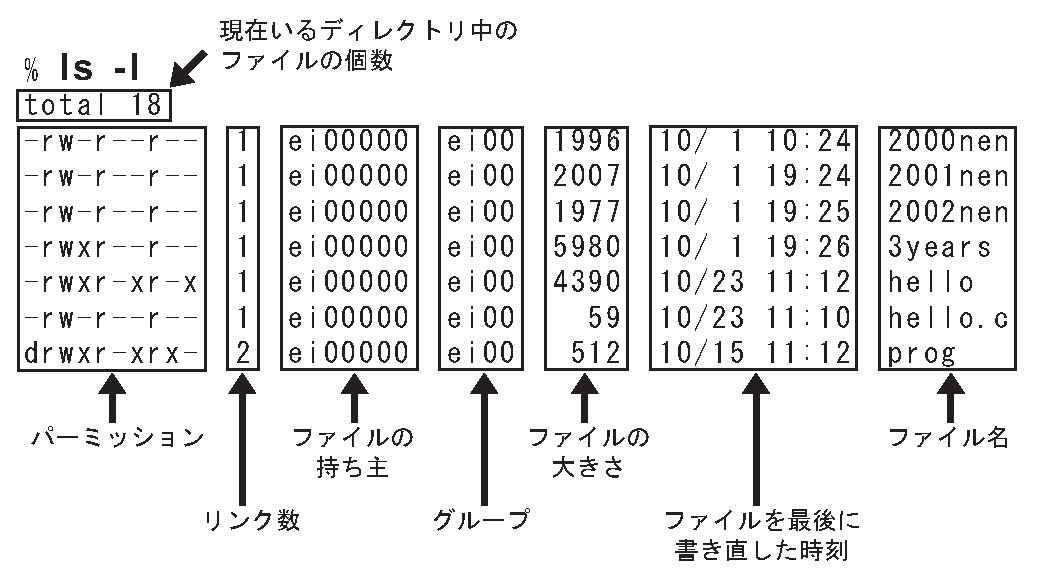
\includegraphics[scale=0.85]{ls-l.eps}}
\caption{\texttt{ls -l} の出力の見方}\label{ls-l}
\end{figure}

この出力の見方は、図 \ref{ls-l} に示した通りである。
ファイルのパーミッションや、持ち主、グループ、ファイルの更新日時などが
表示される。

\subsection{パーミッションの見方}

では次に、具体的にパーミッションの見方を説明しよう。

まず、 UNIX システムでは、
「読める(r: \textbf{r}ead)」「書ける(w: \textbf{w}rite)」
「実行できる(x: e\textbf{x}ecute)」の
 3 種類のパーミッションがある。

例えば、図 \ref{ls-l} を見ると、「\texttt{2000nen}」というファイルの
パーミッションは「\texttt{-rw-r--r--}」と表示されている。
これは、図 \ref{perm1} のように、 4 つのパートに分けて見る。

\begin{figure}[H]
\centering{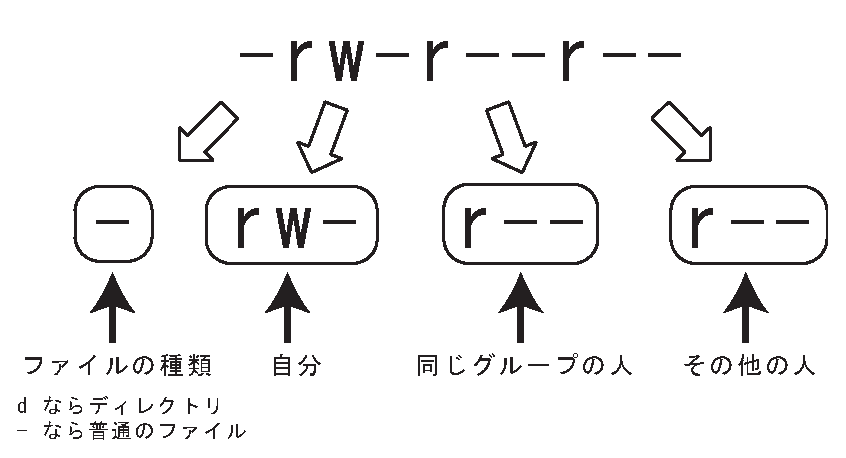
\includegraphics[scale=0.85]{perm1.eps}}
\caption{パーミッションの見方}\label{perm1}
\end{figure}

最初の部分は、ディレクトリか普通のファイルかという区別を表す。
「\texttt{d}」となっていればディレクトリで、
「\texttt{-}」なら普通のファイルである。
例えば「\texttt{-rw-r--r--}」ならファイル、
「\texttt{drwxr-xr-x}」ならディレクトリだ。

\bigskip

次の部分は 3 つで 1 セットになったパーミッションが、 3 つ並んでいる。

最初の 3 つが自分に対するパーミッション、
次の 3 つがファイルのグループに属している人に対するパーミッション、
最後の 3 つがそれ以外の人に対するパーミッションを表している。

\bigskip

 3 つ 1 セットのパーミッションは、次の図 \ref{perm2} のように、
最初から順番に \texttt{rwx} と、 3 つのパーミッションを表している。

\begin{figure}[H]
\centering{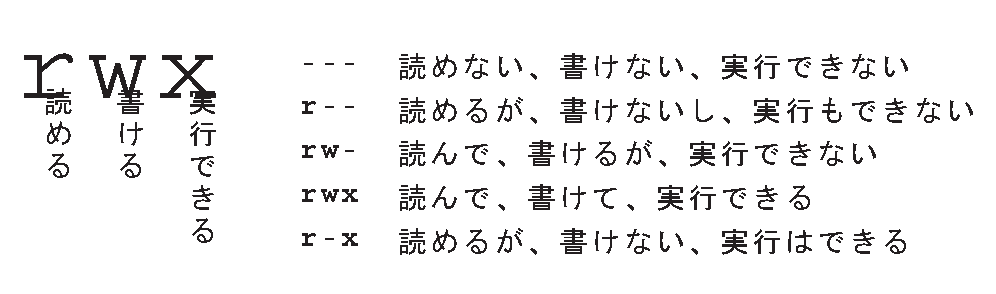
\includegraphics[scale=0.85]{perm2.eps}}
\caption{\texttt{rwx} の見方}\label{perm2}
\end{figure}

 \texttt{r} の部分に、「\texttt{r}」と書いてあれば読めるファイルで、
「\texttt{-}」なら読めないファイルであることを表す。

次の \texttt{w} の部分に、「\texttt{w}」と書いてあれば書き込めるファイル、
「\texttt{-}」なら書けないファイルだ。

 \texttt{x} の部分に、「\texttt{x}」と書いてあれば実行できるファイルで、
「\texttt{-}」なら実行できないファイルだ。
なお、ディレクトリの場合、「\texttt{x}」は中に入ることができるもの、
「\texttt{-}」は入ることができないものを意味する。

\newpage

\subsection{パーミッションの変更: \texttt{chmod}}

このパーミッションを変えるには、 \texttt{chmod} コマンドを使う。
これは、「\textbf{ch}ange \textbf{mod}e -- モード変更」の略である。
 \texttt{chmod} は、次のように使う。
ここでモードというのは、パーミッションを 8 進数に直したものだ。

\begin{coml}{8.5cm}
\texttt{chmod} 「モード」 「ファイル名」
\end{coml}

\subsubsection{モードとは?}

モードについては図 \ref{perm3} で紹介している。
まず、パーミッションは、 \texttt{rwx} の 3 つが並んでいる。
このうち、「\texttt{r}」「\texttt{w}」「\texttt{x}」が書いてあるところを
「1」、「\texttt{-}」になっているところを「0」にして、 2 進数にする。
この 2 進数を、 8 進数に直したものがモードだ。

 8 進数と言うと難しそうに聞こえるかもしれないが、
 1 ケタの 8 進数なので、 10 進数と同じように計算できる。

\medskip

例えば、「\texttt{rw-}」というパーミッションは、 2 進数で書くと「110」だ。
そして、 3 ケタの  2 進数の場合、上の方から順番に、「4 の位」、「2 の位」、
「1 の位」になっている。
よって、「110」は、「4 の位」と「2 の位」が 1 なので、 $ 4+2=6 $、
つまり 8 進数では「6」になる。

\medskip

モードの計算は、このようにそれほど難しくない。
しかし、毎回いちいち計算するのは面倒なので、
よく使うパーミッションと、それをモードに直したものを、
図 \ref{perm4} にあげておいた。

\begin{figure}[H]
\centering{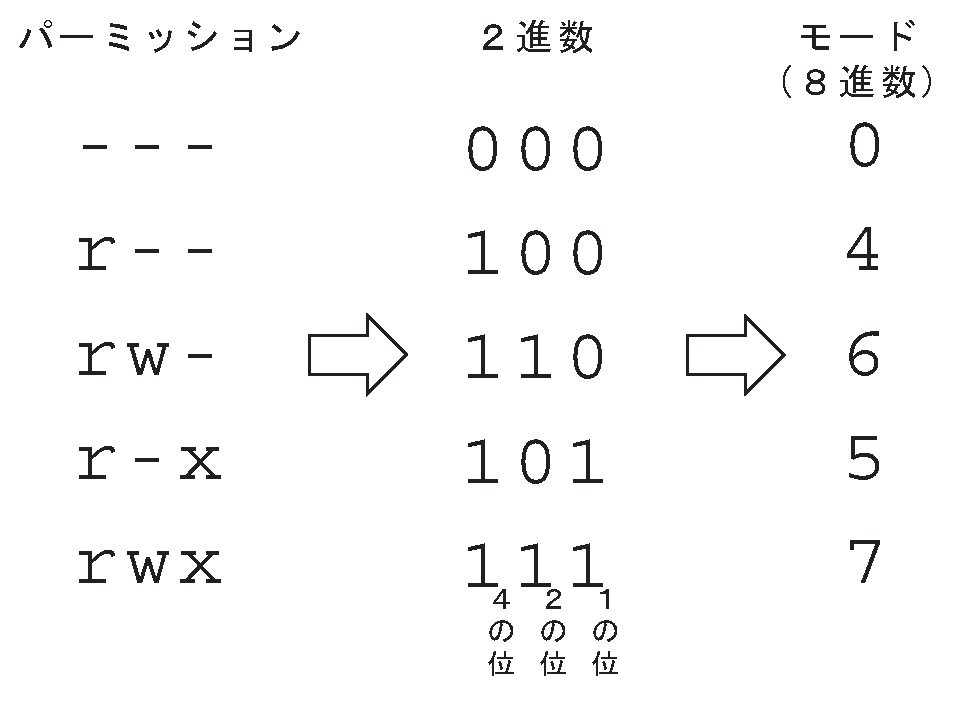
\includegraphics[scale=0.85]{perm3.eps}}
\caption{パーミッションからモードを求める方法}\label{perm3}
\end{figure}

\begin{figure}[H]
\centering{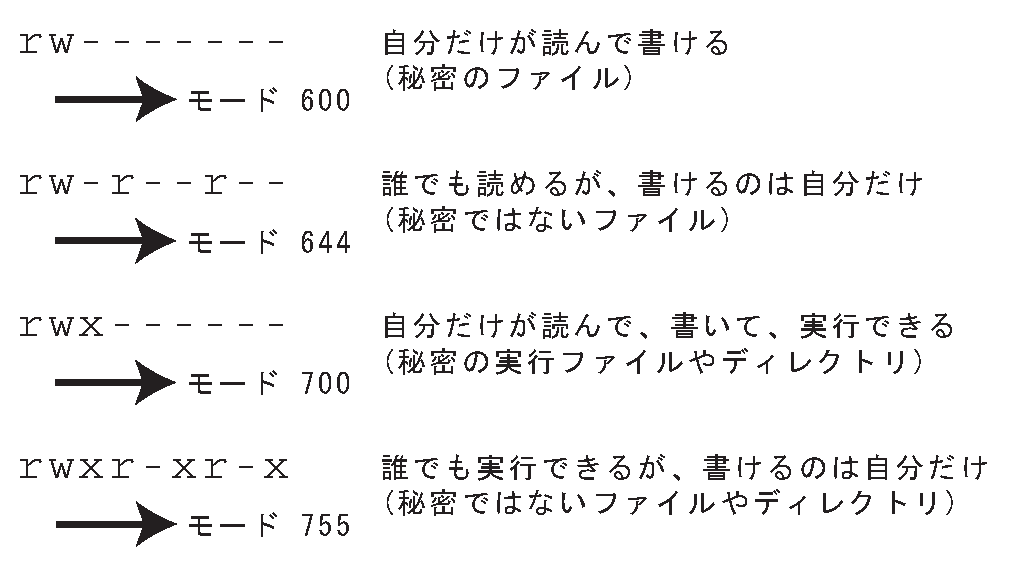
\includegraphics[scale=0.85]{perm4.eps}}
\caption{よく使うパーミッションとそのモード}\label{perm4}
\end{figure}

\subsubsection{実際のパーミッション操作}

では、実際に「\texttt{hello.c}」や「\texttt{hello}」という
ファイルを使って、パーミッションの変更をしてみよう。

\bigskip

まず、「\texttt{hello.c}」と「\texttt{hello}」のパーミッションを
「\texttt{ls -l}」で見てみる。

\begin{progls}
% \slbfl{ls -l}
 [中略]
-rwxr-xr-x  1 ei00000  ei00  4390  10/23 11:12  hello
-rw-r--r--  1 ei00000  ei00    59  10/23 11:10  hello.c
 [中略]
%
\end{progls}

すると「\texttt{hello}」は、誰でも読んで実行できるが、書けるのは自分だけ
ということがわかる。
また、「\texttt{hello.c}」の方は、誰でも読めるが、書けるのは自分だけだ。

\bigskip

ここで「\texttt{hello.c}」を、他人から読めない、
自分だけの秘密のファイルにしてみよう。
自分だけ読み書きできるパーミッションは「\texttt{rw-------}」であり、
モードは「\texttt{600}」になる(図 \ref{perm4} 参照)。
よって、次のようにすればよい。

\begin{progls}
% \slbfl{chmod 600 hello.c}
%
\end{progls}

では、 \texttt{ls -l} で確認してみよう。

\begin{progls}
% \slbfl{ls -l}
 [中略]
-rw-------  1 ei00000  ei00    59  10/23 11:10  hello.c
 [中略]
%
\end{progls}

確かに「\texttt{rw-------}」になっている。
これで、他人からは読めない。

\bigskip

では次に、ちょっとためしに、この「\texttt{hello.c}」を、誰にも読めない、
書けない、実行できないという究極の秘密ファイルにしてみよう。
このパーミッションは「\texttt{---------}」になるので、
モードは「\texttt{000}」である。
というわけで、次のように実行してみよう。

\begin{progls}
% \slbfl{chmod 000 hello.c}
%
\end{progls}

 \texttt{ls -l} で確認すると。

\begin{progls}
% \slbfl{ls -l}
 [中略]
----------  1 ei00000  ei00    59  10/23 11:10  hello.c
 [中略]
%
\end{progls}

では、本当に読んだり書いたりできないか、 Mule を起動して確かめてみよう。

\begin{progls}
% \slbfl{mule hello.c \&}
%
\end{progls}

すると次のように、画面下のミニ・バッファに
「\texttt{File exists, but cannot be read.}
(ファイルはあるけど、読めないよ)」と言われて、
画面には何も表示されないはずだ。

確かに読めないし、書けない。

\begin{figure}[H]
\centering{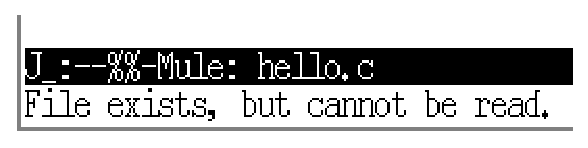
\includegraphics[scale=0.85]{fex-01.eps}}
\end{figure}

もちろん、 \texttt{cat} で中を見ようとしても、
次のように「\texttt{Permission denied} (許可されていません)」
とメッセージが出て、表示されない。

\begin{progls}
% \slbfl{cat hello.c}
cat: hello.c: Permission denied
%
\end{progls}

\bigskip

次に自分だけは読めるが、書けないように変更してみよう。
なお、間違って消したくないファイルは、このように設定しておくとよい。

この場合、パーミッションは「\texttt{r--------}」なので、
モードは「\texttt{400}」だ(図 \ref{perm4} 参照)。
よって、次のようにして変更する。

\begin{progls}
% \slbfl{chmod 400 hello.c}
%
\end{progls}

\texttt{ls -l} で確認すると、

\begin{progls}
% \slbfl{ls -l}
 [中略]
-r--------  1 ei00000  ei00    59  10/23 11:10  hello.c
 [中略]
% 
\end{progls}

これを Mule でいじってみよう。

\begin{progls}
% \slbfl{mule hello.c \&}
%
\end{progls}

すると次の図のように、最初一瞬だけ、画面下のミニ・バッファに
「\texttt{Note: file is write protected} (ファイルは書き込み禁止です)」
と表示される。
そして、ファイルの中身が表示される。

\begin{figure}[H]
\centering{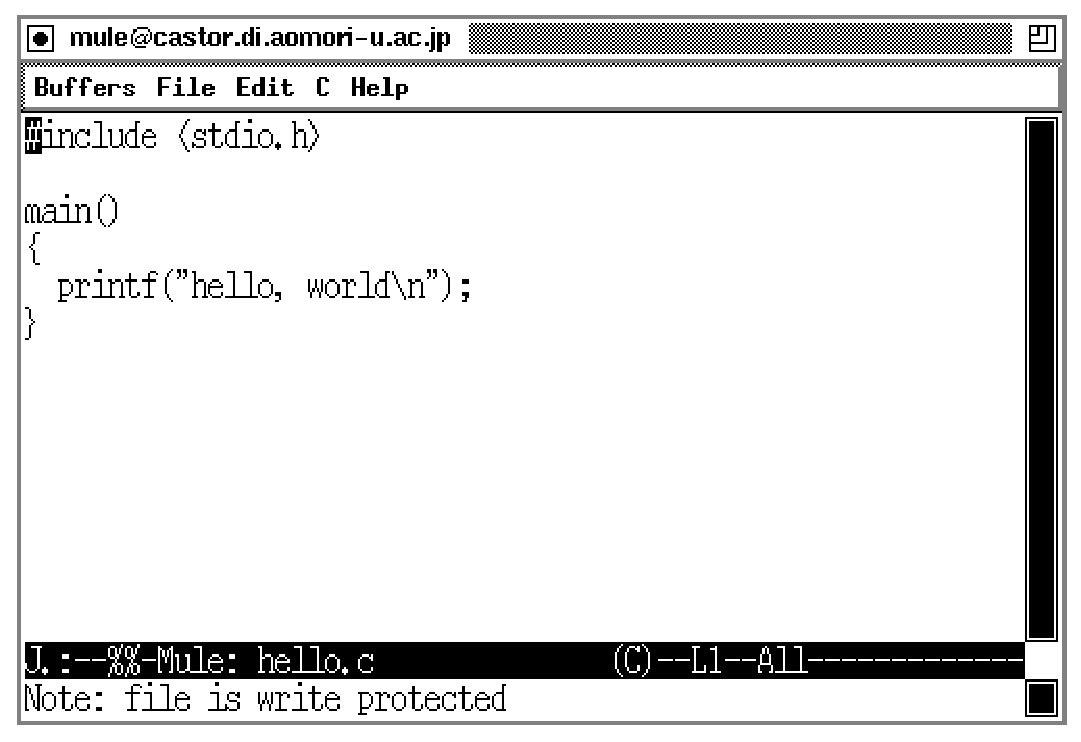
\includegraphics[scale=0.85]{fro-01.eps}}
\end{figure}

ここに、何か文字を入れようとすると、下の図のようにミニ・バッファに
「\verb+Buffer is read-only:+
\verb+#<buffer hello.c>+ (バッファは読むことしかできません)」と表示されて、
結局文字を打てないことがわかるだろう。

\begin{figure}[H]
\centering{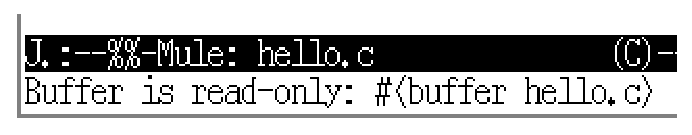
\includegraphics[scale=0.85]{fro-02.eps}}
\end{figure}

\newpage

最後に元にもどしてみよう。
最初のパーミッションは \texttt{rw-r--r--} だったので、
モードは \texttt{644} だ(図 \ref{perm4} 参照)。
そこで、次のようにする。

\begin{progls}
% \slbfl{chmod 644 hello.c}
%
\end{progls}

\texttt{ls -l} で確認すると、確かに元にもどっている。

\begin{progls}
% \slbfl{ls -l}
 [中略]
-rw-r--r--  1 ei00000  ei00    59  10/23 11:10  hello.c
 [中略]
%
\end{progls}

\bigskip

次に「\texttt{hello}」という実行型ファイルのパーミッションを
操作してみよう。
まず、このファイルの現在のパーミッションは次のようになっている。

\begin{progls}
% \slbfl{ls -l}
 [中略]
-rwxr-xr-x  1 ei00000  ei00  4390  10/23 11:12  hello
 [中略]
%
\end{progls}

つまり、誰でも読んで実行できるが、書けるのは自分だけだ。
これを、読み書きに関してはそのままで、誰も実行できないように変更してみよう。
そのようなパーミッションは「\texttt{rw-r--r--}」で、
モードは「\texttt{644}」である(図 \ref{perm4} 参照)。

\begin{progls}
% \slbfl{chmod 644 hello.c}
%
\end{progls}

\texttt{ls -l} で確認してみると、確かに実行できなくなっていることがわかる。

\begin{progls}
% \slbfl{ls -l}
 [中略]
-rw-r--r--  1 ei00000  ei00  4390  10/23 11:12  hello
 [中略]
%
\end{progls}

では、本当に実行できないか、念のため確かめて見よう。

\begin{progls}
% \slbfl{./hello}
./hello: Permission denied.
%
\end{progls}

確かに、「\texttt{Permission denied.}(許可されていません。)」という
メッセージが出て、実行できない。

では、元にもどしてみよう。
最初、パーミッションは「\texttt{rwxr-xr-x}」だった、
よってモードは「\texttt{755}」だ(図 \ref{perm4} 参照)。

\begin{progls}
% \slbfl{chmod 755 hello}
%
\end{progls}

 \texttt{ls -l} で確認する。

\begin{progls}
% \slbfl{ls -l}
 [中略]
-rwxr-xr-x  1 ei00000  ei00  4390  10/23 11:12  hello
 [中略]
\end{progls}

では、実行できるか試して見よう。

\begin{progls}
% \slbfl{./hello}
hello, world
%
\end{progls}

確かに実行できることがわかる。

\section*{この章で紹介したコマンド}

\begin{center}
\begin{minipage}{13cm}
\begin{itembox}[l]{パーミッションの操作}
\begin{description}
\item[\texttt{chmod} :] パーミッションの変更

使い方: \texttt{chmod} 「モード」 「ファイル名(複数指定可)」
\end{description}
\end{itembox}
\end{minipage}
\end{center}

\begin{center}
\begin{minipage}{13cm}
\begin{itembox}[l]{C コンパイラ}
\begin{description}
\item[\texttt{cc} :] C コンパイラ

使い方: \texttt{cc}~~~-o~~~「実行型ファイル名」~~~「ソースのファイル名」
\end{description}
\end{itembox}
\end{minipage}
\end{center}

%\newpage
%{~}
